\section{Resultados y gráficos}

\subsection{Resultados (Ejercicio 1)}
\label{Resultados1}

\paragraph{}
El programa \textit{input\_gen1} fue desarrollado para poder generar diversos casos de pruebas en los que \textit{n} adopte distintos valores\footnote{Aclaración: En todos los casos b es un numero entre 0 y 1.000.000}. A continuación se describen cuáles son esos casos y se explica brevemente que se esperaba observar en cada uno de ellos.
	\begin{itemize}
		\item[\texttt{a.-}]{\texttt{Casos con n entre 1.000.000 y 1000.000.000:} \\
		Se pensó en este tipo de casos para poder evaluar el comportamiento del algoritmo frente a valores de \textit{n} muy grandes.}
		\item[\texttt{b.-}]{\texttt{Casos con n entre 1 y 1.000.000:} \\
		Se pensó en este tipo de casos para poder evaluar el comportamiento del algoritmo frente a valores de \textit{n} bastante acotados.}
		\item[\texttt{c.-}]{\texttt{Casos con b multiplo de n , con n entre 1 y 1.000.000:} \\
		Se pensó en este tipo de casos para poder observar la situación más favorable, en la cual el algortimo solo debe efectuar una operación que es la de ver si $b\ mod\ n\ =\ 0$ y en ese caso devolver 0.}
   		\item[\texttt{d.-}]{\texttt{Casos con n = $2^k - 1$, con k entre 2 y 30:} \\
		Se pensó en este tipo de casos para poder observar el comportamiento del algoritmo en la situación más desfavorable. Esta es en la cual al realizar la división enterda del exponente de \textit{b} por 2 el resultado es siempre un número impar, por lo cual el algoritmo entra por en el último \textit{else} que es el bloque de código con mayor número de operaciones.} 
		\item[\texttt{e.-}]{\texttt{Casos con n primo con n entre 1 y 1000.000.000:} \\
		Se pensó en este tipo de casos para poder evaluar el comportamiento del algoritmo frente a valores de \textit{n} primos.}
	\end{itemize}  

\paragraph{}
Mediante cada uno de estos casos se buscó estudiar el comportamiento del algoritmo y medir su complejidad real, valiéndose para ello del conteo de la cantidad de operaciones que realiza el algoritmo para resolver el problema. No obstante, previo a la experimentación, se formularon varias hipótesis en cuanto a qué era esperable observar en cada caso en particular:
	\begin{itemize}
		\item[1)]{En el caso \texttt{c}, dado que el algoritmo realiza 2 asignaciones y una única cuenta (la de calcular el resto de \textit{b} módulo \textit{n}), resulta esperable que la complejidad real sea de valor constante 3.}
		\item[2)]{Para los casos \texttt{a} y \texttt{b} sabemos que la complejidad teórica del algoritmo es \Ode{log_2(n)}. No obstante, como los \textit{n's} del caso \texttt{a} son del orden de $10^9$, mientras que los \textit{n's} del caso \texttt{b} son del orden de $10^6$ cabría esperar que la cantidad de operaciones para los \textit{n's} del caso \texttt{a} sean mayores que los del caso \texttt{b}}. 
		\item[3)]{El caso de \texttt{e} es análogo al de \texttt{a}, ya que en ambos casos los \textit{n's} son del orden de $10^9$, y la complejidad teórica del algoritmono varía. Sin embargo, se podría suponer a priori que por tratarse \textit{n's} primos, la cantidad de operaciones del caso \texttt{e} sea ligeramente mayor a la cantidad de operaciones del caso \texttt{a}.}
		\item[4)]{Por último, en el caso \texttt{d}, cada llamado recursivo del algoritmo siempre ingresa al blóque de código de los exponentes impares. Por ende, como realiza exactamente q operaciones $log_2$(n) veces es presumible que \texttt{d} sea el peor caso de este algoritmo.}
	\end{itemize}

\paragraph{}
Para la experimentación con el programa se generó un archivo con 150 pares de números $b,\ n \in \nat$ para cada uno de los casos anteriores. Luego, se los procesó corriendo el programa \textit{ejercicio\_1} y cada archivo de entrada obtuvo su correspondiente archivo \textit{"NombreDeArchivo.out"} y su correspondiente archivo \textit{"NombreDeArchivo\_grafico.out"} en el cual se registraron los valores de \textit{n} y la cantidad de operaciones que realizó el algoritmo en ese caso. Finalmente, haciendo uso de esos archivos se generaron, usando el programa de análisis gráfico \textit{QtiPlot}, diversos gráficos de \textit{n} vs. \textit{cantidad de operaciones} en los cuales se contrasta la curva de resultados con una función $f: \nat \rightarrow \real / f(n)\ =\ c.log_2(n)$, $c \in \real^+$ para poder estudiar si la complejidad real se ajusta a la complejidad teórica.\\

\paragraph{}
A continuación se presentan los gráficos realizados para cada caso:

	%grafico de a.in
	\begin{table}[ht]
		\centering 
			\begin{tabular}{c}
				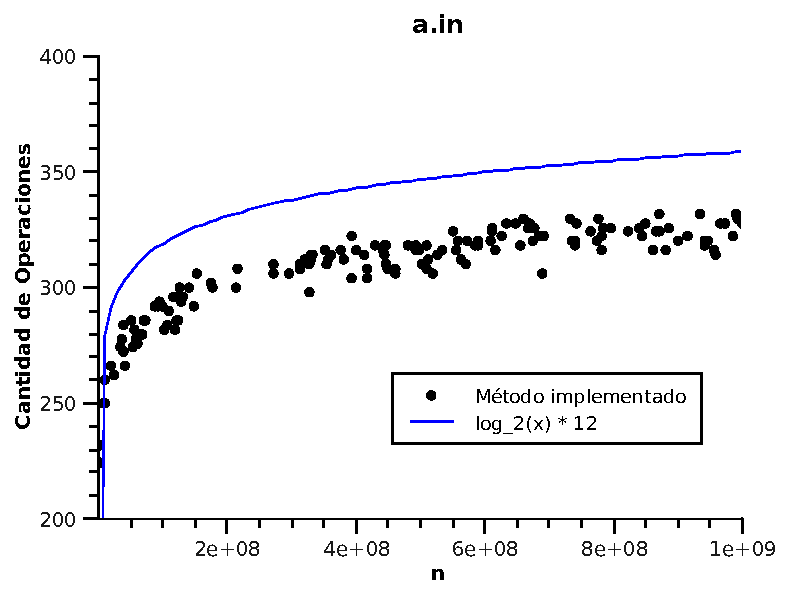
\includegraphics[scale = 0.8]{./../ej1/tests/a.pdf}
			\end{tabular}
			\caption{.}
			\label{grafico1} 
	\end{table}

	%grafico de b.in
	\begin{table}[ht]
		\centering 
			\begin{tabular}{c}
				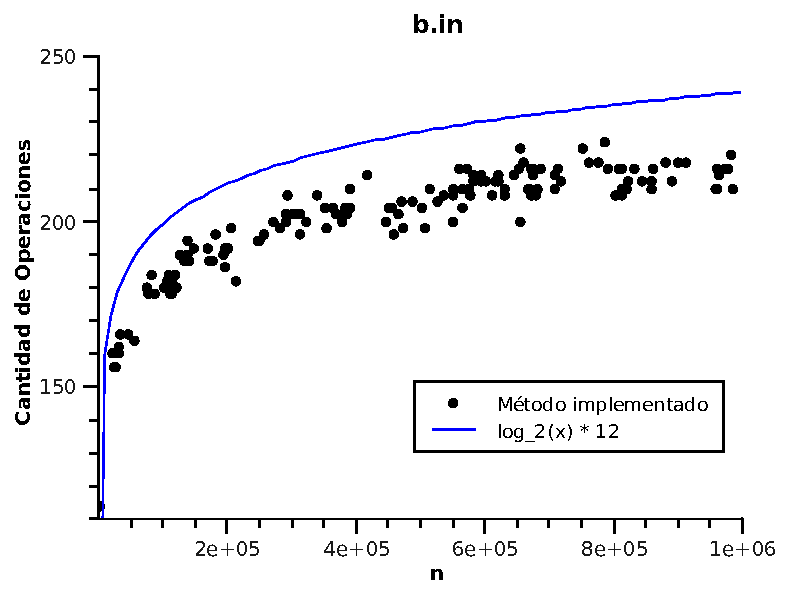
\includegraphics[scale = 0.8]{./../ej1/tests/b.pdf}
			\end{tabular}
			\caption{.} 
			\label{grafico2} 
	\end{table}

	% grafico de c.in
	\begin{table}[ht]
		\centering 
			\begin{tabular}{c}
				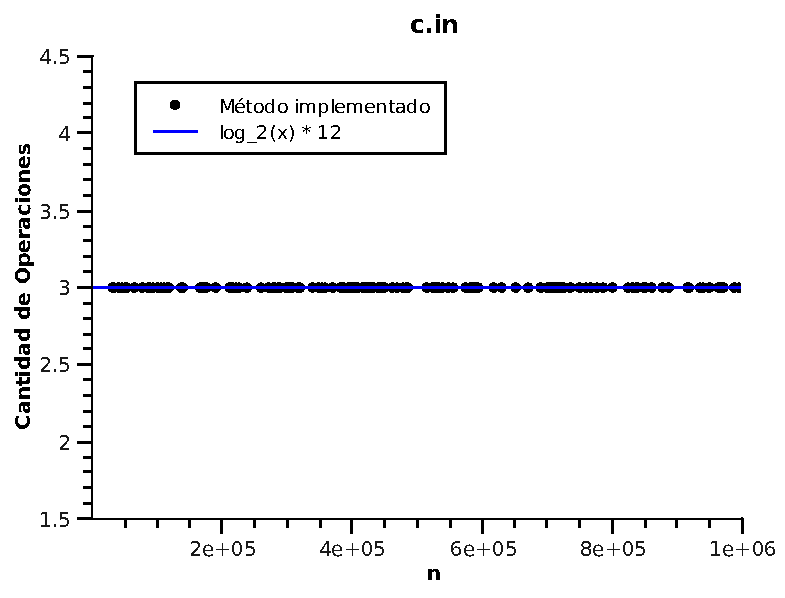
\includegraphics[scale = 0.8]{./../ej1/tests/c.pdf}
			\end{tabular}
			\caption{.}
			\label{grafico3} 
	\end{table}

	%grafico de d.in
	\begin{table}[ht]
		\centering 
			\begin{tabular}{c}
				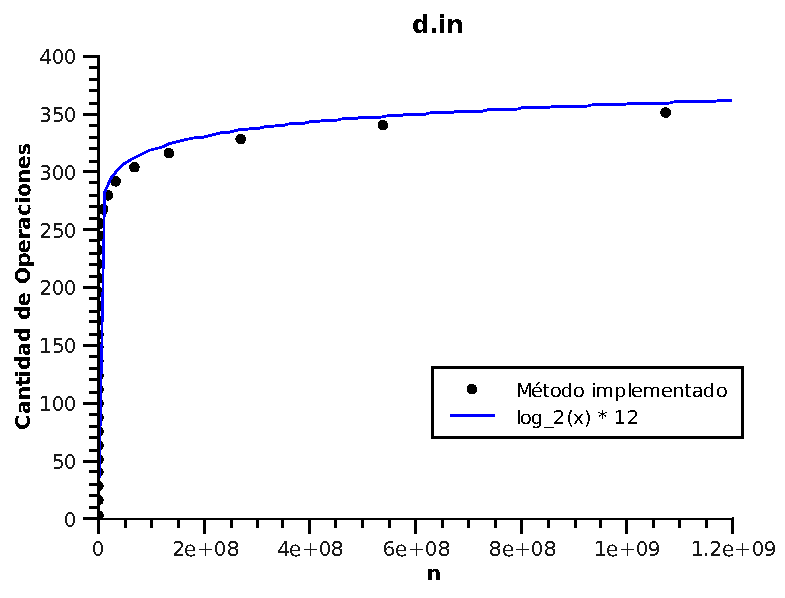
\includegraphics[scale = 0.8]{./../ej1/tests/d.pdf}
			\end{tabular}
			\caption{.} 
			\label{grafico4} 
	\end{table}

	%grafico de e.in
	\begin{table}[ht]
		\centering 
			\begin{tabular}{c}
				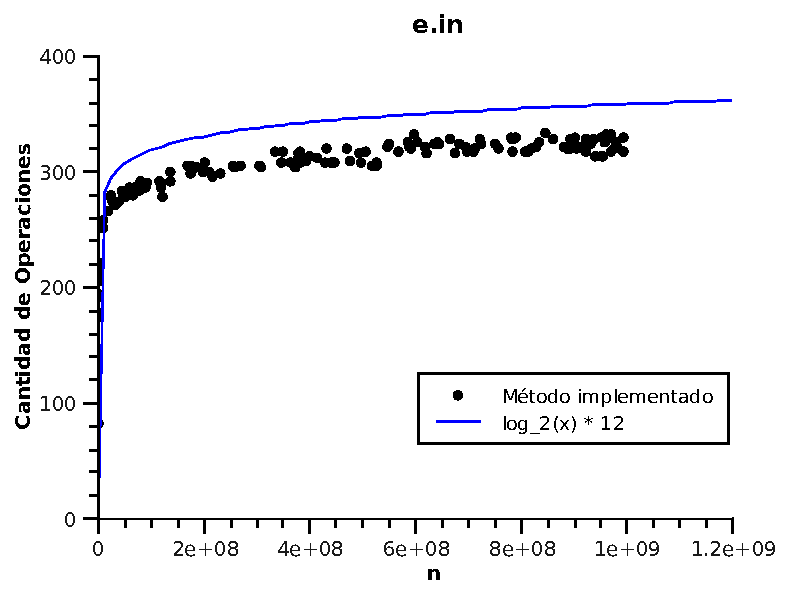
\includegraphics[scale = 0.8]{./../ej1/tests/e.pdf}
			\end{tabular}
			\caption{.}
			\label{grafico4} 
	\end{table}
	

\newpage
\newpage
\newpage
\subsection{Resultados (Ejercicio 2)}
\label{resultadosej2}


	\begin{table}[h!] %ubicacion de la tabla
		\centering %centra la tabla
			\begin{tabular}{c}
				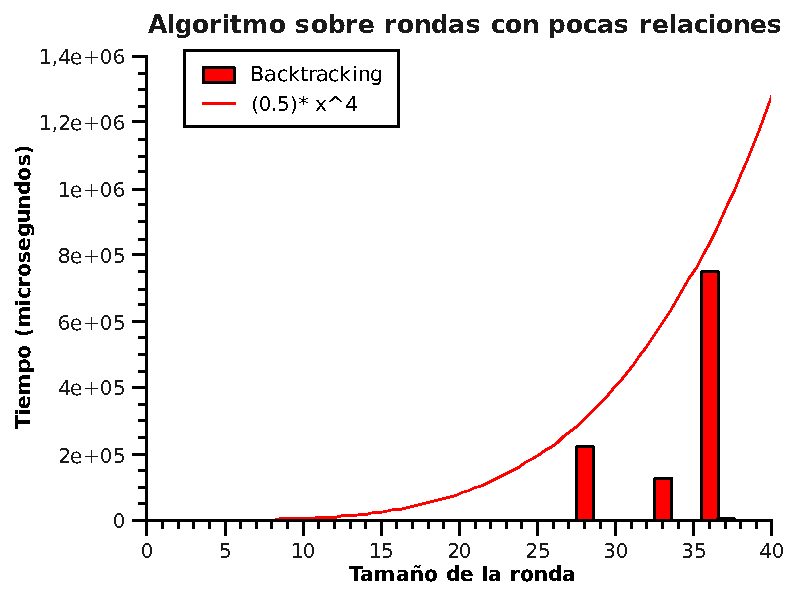
\includegraphics[scale=0.7]{../Ej_2/Otros/Graficos/Graph10-1.pdf} \\
				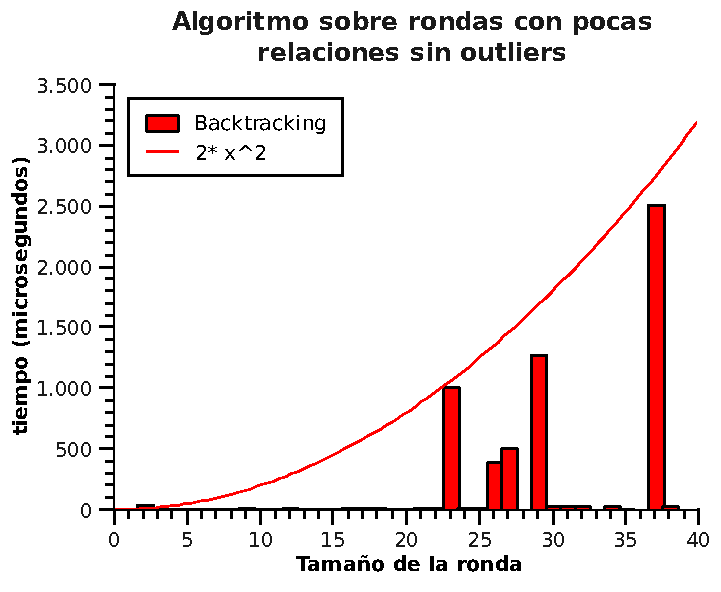
\includegraphics[scale=0.7]{../Ej_2/Otros/Graficos/Graph10-2.pdf}
				\end{tabular}
				\caption{Rondas con pocas relaciones: Estos graficos muestran la desigualdad entre tiempos de resolución para rondas es donde es complicado encontrar la solución. Se ve que quitando unos pocos outliers, los tiempos se encuentran en otros ordenes. Para ver este suceso, basta con obvservar las escalas de tiempo (en un gráfico se mueve entre 0 y 3500 microsegundos, y en la que posee outliers entre 0 y 1400000 microsegundos.) o también se puede observar las funciones que se utilizaron para dar cuenta de las dimensiones (en una comparada con $0.5*x^4$ y en la otra con $2x^2$).} %titulo de la tabla
				\label{tiempoEj2a} %con esto puedo referenciar a la tabla \ref{Tiempo metodos}
	\end{table}

	\begin{table}[h!] %ubicacion de la tabla
		\centering %centra la tabla
			\begin{tabular}{c}
				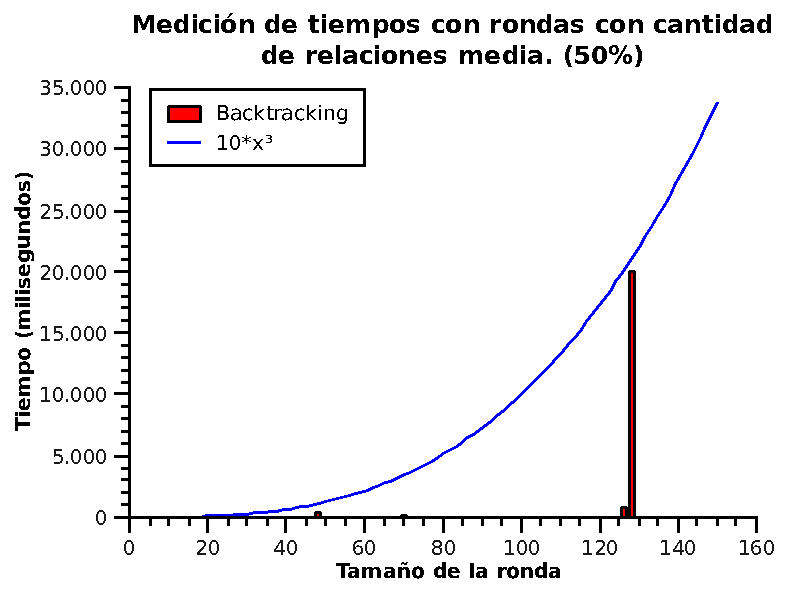
\includegraphics[scale=0.7]{../Ej_2/Otros/Graficos/Graph50-1.pdf} \\
				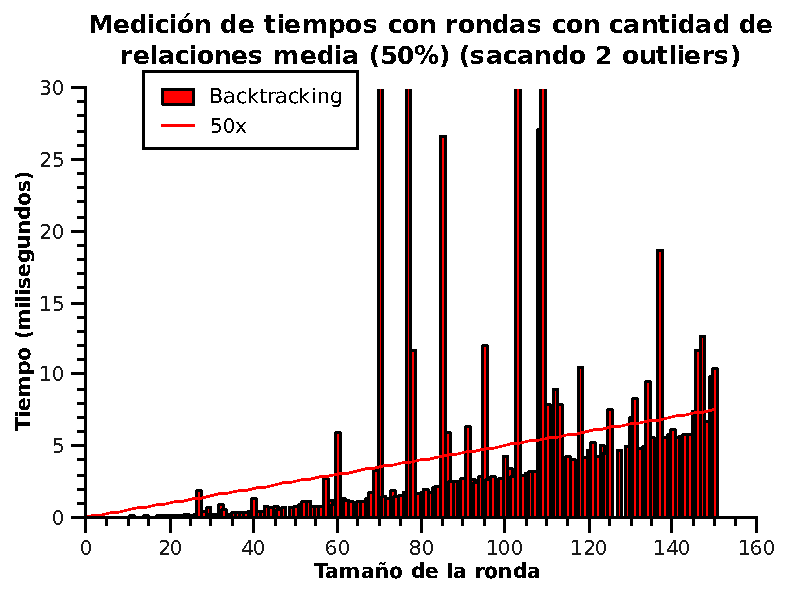
\includegraphics[scale=0.7]{../Ej_2/Otros/Graficos/Graph50-2.pdf}
			\end{tabular}
			\caption{Rondas con una cantidad media de relaciones: En estos se puede observar como 2 outliers destruyen el caso promedio que se venia dando en el tiempo de resolución del algoritmo, pasando de graficos que se comparan con $10*x^3$ contra otro que compara con $50*x$, es decir, para rondas donde hay buenas probabilidades de que se pueda formar, el algoritmo parecería comportarse linealmente, pero claramente es una ilusión.} %titulo de la tabla
			\label{tiempoEj2b} %con esto puedo referenciar a la tabla \ref{Tiempo metodos}
	\end{table}

\begin{table}[h!] %ubicacion de la tabla
\centering %centra la tabla
\begin{tabular}{c}
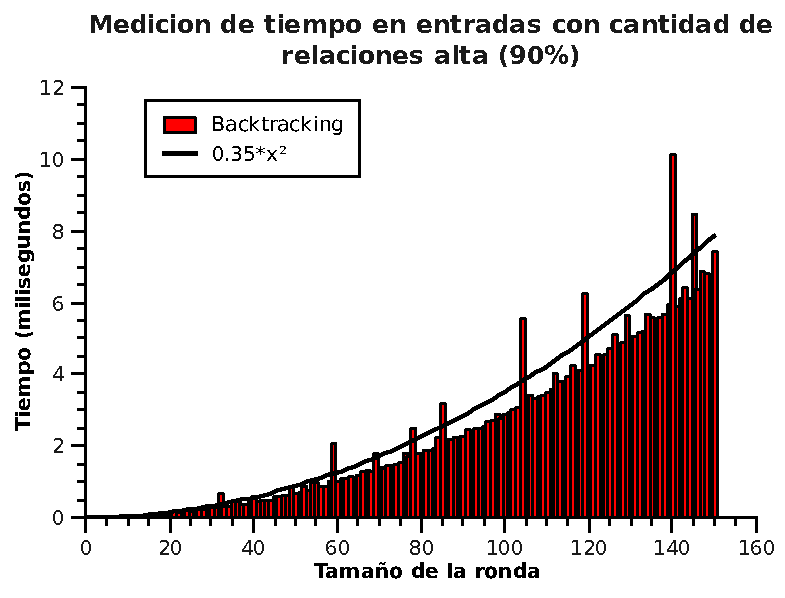
\includegraphics[scale=0.7]{../Ej_2/Otros/Graficos/Graph90.pdf} \\
\end{tabular}

\caption{Rondas con una cantidad alta de relaciones: Cuando es muy poco probable que NO se pueda armar una ronda, el algoritmo y sus mejoras claramente funcionan bien (polimomial), como es el caso de este gráfico. Esto se debe a las propiedades del backtracking y a las mejoras implementadas.} %titulo de la tabla
\label{tiempoEj2c} %con esto puedo referenciar a la tabla \ref{Tiempo metodos}
\end{table}

\newpage
\subsection{Resultados (Ejercicio 3)}
\label{resultadosej3}

\paragraph{}
De la sección Explicación y de un análisis más minucioso del pseudocódigo, se desprende como algunas hipótesis
 que el peor caso se da cuando hay muchos trabajadores dispersos durante todo el día, es decir, si todos los horarios de salida y entrada entre dos trabajadores cualesquiera son disjuntos.

\paragraph{}
Para poder analizar el comportamiento del algoritmo implementado, se procedió a realizar un programa que genere distintas entradas, de acuerdo a distintos criterios que nos parecieron relevantes remarcar.\\
De esta manera, se utilizaron dos formas distintas de generar un archivo de entrada. Una de ellas se corresponde a una entrada completamente azarosa, a modo de analizar el comportamiento del algoritmo para una extensa cantidad de casos distintos. La segunda, trata de plasmar en sus casos la hipótesis de peor caso planteada en el párrafo anterior.

\paragraph{}
A continuación se adjuntan los gráficos provenientes de analizar los casos antes planteados. Están agrupados de a pares, a modo de mostrar más claramente la diferencia en la complejidad de cada caso.
	\begin{table}[h!] %ubicacion de la tabla
		\centering %centra la tabla
		\begin{tabular}{c}
			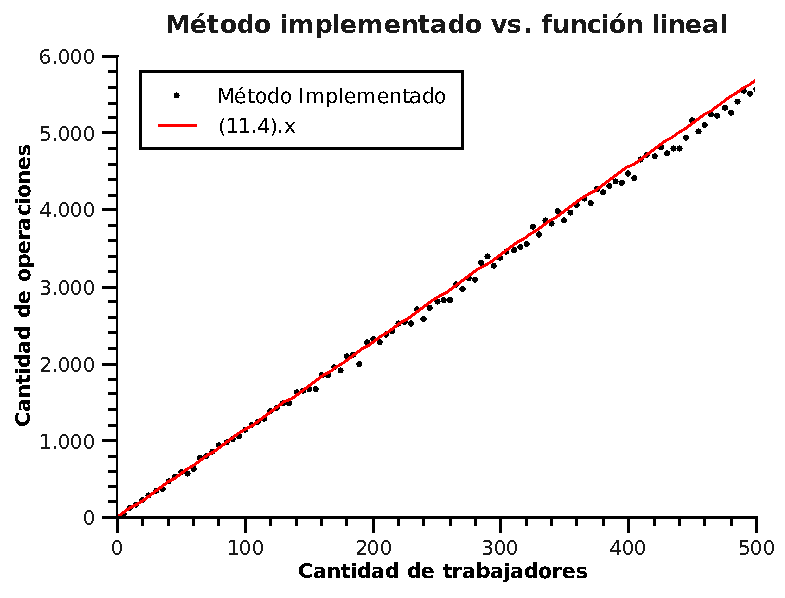
\includegraphics[scale=0.7]{../ej3/graficos/contarOp1.pdf} \\
			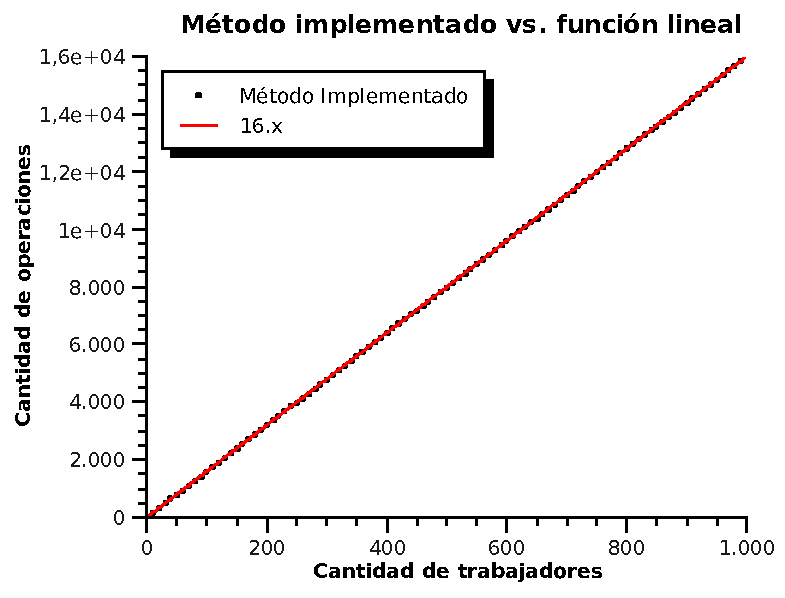
\includegraphics[scale=0.7]{../ej3/graficos/contarOp5.pdf}
		\end{tabular}
		\caption{Muestran el comportamiento de la cantidad de operaciones contra la cantidad de trabajadores. El primer gráfico proviene de una entrada hecha al azar. El segundo proviene de evaluar el comportamiento del algoritmo para el peor caso.} %titulo de la tabla
		\label{cantOpEj3} %con esto puedo referenciar a la tabla \ref{Tiempo metodos}
	\end{table}

	\begin{table}[h!] %ubicacion de la tabla
		\centering %centra la tabla
		\begin{tabular}{c}
			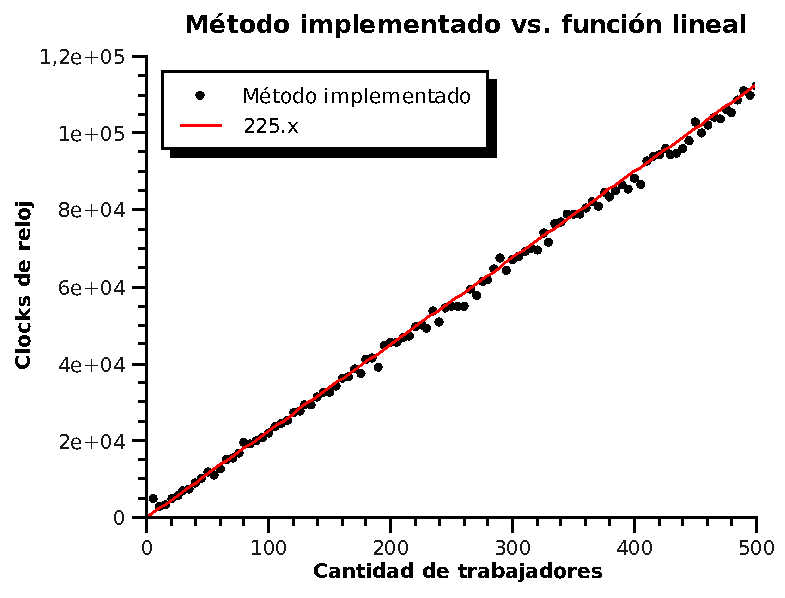
\includegraphics[scale=0.7]{../ej3/graficos/clocks1.pdf} \\
			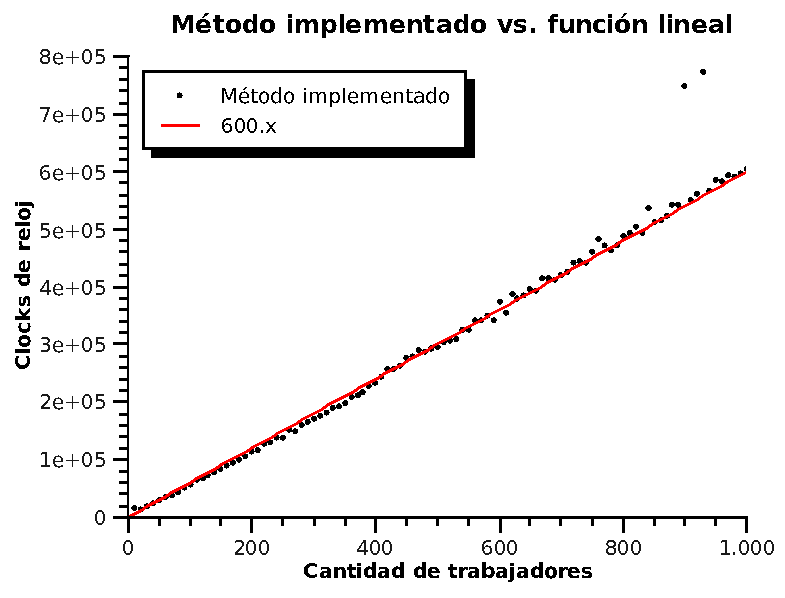
\includegraphics[scale=0.7]{../ej3/graficos/clocks5.pdf}
		\end{tabular}
		\caption{Muestran el comportamiento de la cantidad de ticks de reloj contra la cantidad de trabajadores. El primer gráfico proviene de una entrada hecha al azar. El segundo proviene de evaluar el comportamiento del algoritmo para el peor caso.} %titulo de la tabla
			\label{clocksEj3} %con esto puedo referenciar a la tabla \ref{Tiempo metodos}
	\end{table}

	\begin{table}[h!] %ubicacion de la tabla
		\centering %centra la tabla
		\begin{tabular}{c}
			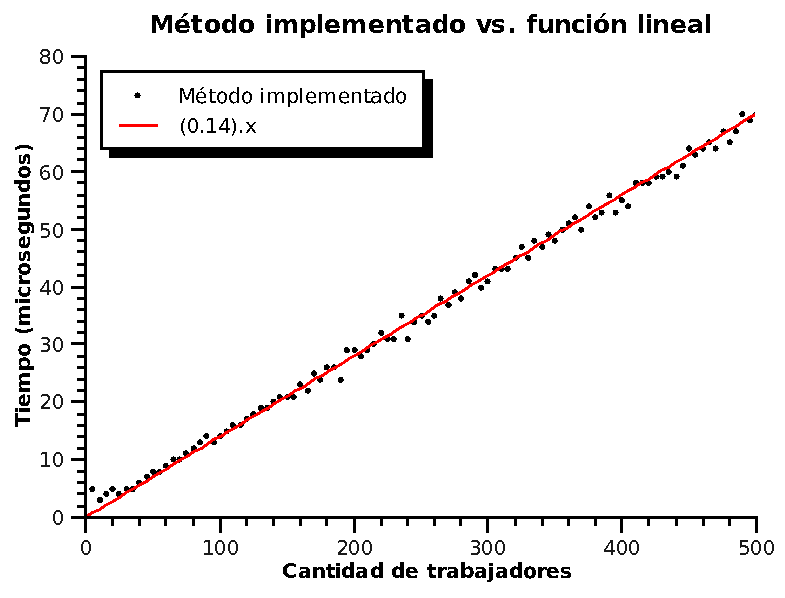
\includegraphics[scale=0.7]{../ej3/graficos/tiempo1.pdf} \\
			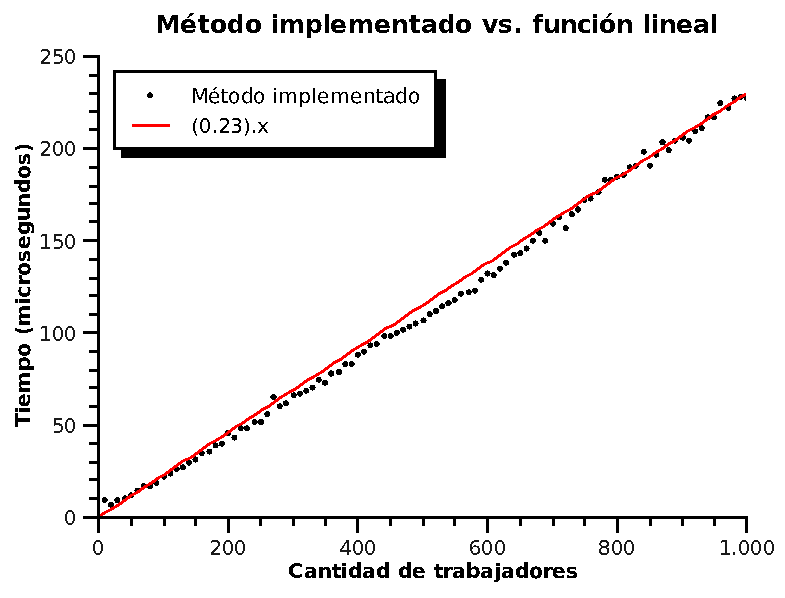
\includegraphics[scale=0.7]{../ej3/graficos/tiempo5.pdf}
			\end{tabular}
		\caption{Muestran el comportamiento de la cantidad de microsegundos contra la cantidad de trabajadores. El primer gráfico proviene de una entrada hecha al azar. El segundo proviene de evaluar el comportamiento del algoritmo para el peor caso.} %titulo de la tabla
		\label{tiempoEj3} %con esto puedo referenciar a la tabla \ref{Tiempo metodos}
	\end{table}